\fenicschapter{Simulations of transitional flows}{Mikael Mortensen, Kent Andr\'{e} Mardal, etc.}

\index{important term}

\newcommand{\Hset}{FIXME: This is undefined!}
\newcommand{\Nset}{FIXME: This is undefined!}

%------------------------------------------------------------------------------
\section{Introduction}
The purpose of this work is to validate Navier-Stokes (NS) solvers implemented in FEniCS for unstable, transitional flows. Solvers for the NS equations have already been discussed in the benchmark chapter \cite{nsbench} for laminar flows. In this chapter focus is put more directly on flow energy and energy conservation, features of primary importance in turbulence applications. We emphasize the treatment of the nonlinear convection term, where various forms (standard, divergence and skew-symmetric) are implemented and tested for both accuracy and stability. The algorithm chosen to advance the momentum and pressure in time is a fractional step approach that is memory efficient, but admits a splitting error due to the uncoupling of velocity and pressure. The significance of this splitting error is validated through comparison with a more accurate fully coupled solver that, due to its higher memory cost, is less suited for large-scale turbulence applications. The performance of the solvers is validated with the one-dimensional Burger's equation, the Orr-Sommerfeld perturbation in two dimensions and finally the full-blown three-dimensional unstable and transitional Taylor-Green vortex.

The solvers and problems are implemented to fit in the problem solving environment described in the benchmark chapter \cite{nsbench}. Source code can be found in the folder \cite{folder}.

\section{Background}

The Navier-Stokes (NS) equations (directly derivable from Newton's second law utilizing the continuum hypothesis) represent a differential form of the principle of conservation of mass and momentum. It governs both laminar and turbulent fluid motion in three-dimensional space and time for incompressible and compressible fluids. There are no closed form analytical solutions to the NS equations and the study of fluid dynamics thus relies heavily on numerical solutions.

For incompressible Newtonian fluids the NS equations read
% The Navier-Stokes (NS) equations are a differential form of the conservation laws for mass and momentum that governs the motion in time \textit{t} of Newtonian incompressible fluids. In the event that body (volumetric) forces $\text{f}$ also act on the fluid element, the momentum concervation law becomes a balance law and the equations read
\begin{align}
 \frac{\partial \vec{u}}{\partial t}+\vec{u}\cdot \nabla \vec{u} &= \nu \nabla^2 \vec{u} -\frac{1}{\rho} \nabla p +\text{f}, \label{eq:NS}\\
 \nabla \cdot \vec{u} &=0.
 \label{eq:cont}
\end{align}
Here $\vec{u}(\text{x},t)$ is the velocity vector, $\text{x}$ is the Cartesian coordinate vector, $\nu$ the kinematic
viscosity ($\mu/\rho$), $\rho$ density, $\mu$ molecular viscosity, $p(\text{x},t)$ pressure, and the volumetric body forces is represented with \textbf{f} (e.g., the gravitational force or the Coriolis forces associated with the imposition of frame rotation). In the absence of viscosity the principle of conservation of energy can also (in addition to mass and momentum) be directly imposed on the NS equations. This particular property is especially important for turbulent flows, since a fundamental feature of turbulence is that kinetic energy is extracted from the flow system and eventually converted into internal energy (heat) by the action of viscosity (rate of dissipation). The largest and most energetic turbulence structures are primarily responsible for efficient mixing of momentum and scalars. These structures are by a series of instability processes broken down to smaller and smaller spatial scales and eventually dissipated into heat. The conservation of kinetic energy (in the absence of viscosity) is thus an important feature of turbulent fluid flows which is formally consistent with the NS equations. Unfortunately, though, this feature is not necessarily retained by the numerical scheme used to solve the discretized NS equations numerically. A numerical method can be both dissipative and dispersive, recognized for example by the order of the derivative in the truncation error of Taylor expansions. A numerical scheme with even order derivatives in truncated terms is dissipative, whereas odd derivatives lead to dispersion.
% Here $\vec{u}(\text{x},t)$ is the velocity vector, $\text{x}$ is the Cartesian coordinate vector, $\nu$ the kinematic viscosity, $\rho$ density and $p(\text{x},t)$ pressure. The equations govern both laminar and turbulent flows. In addition to conserving mass and momentum, it can also be shown that the equations should conserve kinetic energy (i.e., the energy of the velocity fluctuations) in the absence of viscosity. The kinetic energy and its rate of dissipation are usually considered the most important features of a turbulent flow. For exaIt is therefore umple, it is widely recognized that the energetic large-scale turbulent eddies are responsible for efficient distribution of momentum (mixing), whereas small-scale eddies lead to dissipation of energy as heat.
% %It is, for example, the rate of dissipation that limits the rate of chemical reactions in turbulent non-premixed combustion; and due to dissipation, the drag will be higher in a turbulent than laminar flow, when both are exposed to the same mechanical energy.
% Energy conservation is a consequence of the NS equations, but unfortunately this feature is not necessarily respected by numerical schemes used to solve them. A numerical method can be both dissipative and dispersive, recognized for example by the order of the derivative in the truncation error of Taylor expansions. A numerical scheme with even order derivatives in truncated terms is dissipative, whereas odd derivatives lead to dispersion. %In turbulent or transitional flows the real physical dissipation caused by the fluid viscosity can be very small far away from solid obstacles or walls. The physical dissipation may as such easily become comparable to the numerical dissipation and it is advantages or some times even necessary to use disspation-free numerical schemes.


The often used terminology Direct Numerical Simulations (DNS) should be understood as the three-dimensional and time dependent numerical simulations of the NS equations that resolve all information (all turbulence scales) and that have negligible numerical dissipation (artificial viscosity) and dispersion. For this reason DNS are often performed with highly accurate spectral (Fourier) methods \cite{Canuto88} in homogeneous flows or higher-order central finite differences or spectral element methods \cite{semtex} for more geometrical flexibility in inhomogeneous flows. The results of carefully executed DNS have in the fluid mechanics community the same status as carefully executed experiments. Unfortunately, though, DNS are very demanding of computer resources. A good part of the expense is incurred in capturing the smallest scales of turbulence, i.e., the scales that are responsible for dissipating energy. Yet another complication in non-periodic flows is to describe inflow and outflow boundary conditions which are consistent with the NS equations.

The computational cost of DNS can (at the expense of accuracy) be reduced by capturing only the largest scales and using a dissipative model in place of the smaller eddies (to try and make up for the loss of accuracy). This method is referred to as Large Eddy Simulations (LES) and it too requires the three-dimensional and time dependent solution. To the extent that the dissipative model does not contaminate the large scales, LES can provide NS simulations of satisfactory accuracy for many purposes. However, the results depend inherently on the grid, because the grid independent solution is nothing but the DNS solution that one in most cases cannot afford. Finding the best possible compromise between efficiency and accuracy is the ongoing dilemma for LES-practitioners.

Laminar flows may under the right circumstances undergo transition to turbulence. The transition can be triggered by several factors, but the physical process are not yet fully understood for many cases. At the turn of the 19'th century Osbourne Reynolds discovered that for cylindrical pipes the transition to turbulence occurred at a Reynolds number of 2300 ($Re=U\cdot h/\nu$, where $U$ is the average velocity and $h$ half the pipe diameter). Later, with very carefully executed experiments in highly smooth pipes, scientists have been able to increase this number considerably, revealing that velocity is not really the triggering factor, even though there clearly is a strong correlation (follows since as the Reynolds number increases, the stabilizing viscous damping term becomes comparatively less than the unstable nonlinear convection term.) Another example of transition can be found in the wakes downstream bluff bodies placed in an incoming laminar flow. Here the transition is promoted by the strong shear layer formed by the recirculation region aft the body. In any case, in order for transition to occur, imposed disturbances triggered by, e.g., obstacles, a sudden pressure fluctuation, or even a soundwave, must grow and become unstable and finally chaotic. By introducing systematic perturbation of the NS equations one can study these phenomena and watch how they experience resonance and grow or gracefully die. Here, the numerical scheme will be of utmost importance to the experiment, because a dissipative scheme will damp (kill) the imposed perturbations.

The most famous early work aimed to study perturbations of the NS equations was conducted more than 100 years ago by William McFadden Orr and Arnold Sommerfeld. The epitome of their analytical work is the celebrated Orr-Sommerfeld equation, which is an eigenvalue problem describing the linear two-dimensional modes of disturbance to a viscous parallel shear flow. Although the Orr-Sommerfeld equation only represents one simple class of laminar-to-turbulence transition, it constitutes a powerful method to assess numerical schemes since it provides an analytical transient solution to the NS equations that remains non-trivial for long integration times. The Orr-Sommerfeld testcase will be further discussed in Sec. \ref{sec:OS}, but first we need to turn our attention to the NS solvers, the numerical methods and their implementation in FEniCS.

\section{Numerical method and energy conservation}
\label{sec:Numerical}
In this section we will discuss both the spatial and temporal discretizations of the Navier-Stokes (NS) equations and special attention will be focused on the nonlinear convection term. Furthermore, since the NS equations represent a system of equations, we will discuss both a fully coupled method where $\vec{u}$ and $p$ are solved simultaneously and a fractional step method that solves for the pressure and velocity in a segregated (non-coupled) manner.

\subsection{Convection}
\label{sec:Convection}
Let $\Omega \subset \Rset^d$ be an open and bounded region in $\Rset^d$, where $d$ is the number of spatial dimensions, with smooth boundary $\Gamma$ and points denoted by $\vec{x}\in \overline{\Omega}=\Omega \cup \Gamma$. The $L_2(\Omega)$ inner product of vectors or matrix fields on $\Omega$ is then denoted as
\begin{equation}
 \bigl( \vec{a},\vec{u} \bigr) = \int_{\Omega} \vec{a}\cdot \vec{u}\, d\Omega,
 \label{eq:L2}
\end{equation}
where $\vec{a}$ and $\vec{u}$ are arbitrary vector fields on $\Omega$. The associated $L_2$-norm is denoted by $\| \cdot \| \equiv \sqrt{\left( \cdot, \cdot \right)}$. Furthermore, let \Hset be the space of $L_2(\Omega)$-smooth vector fields tangent to the boundary $\Gamma$ and denote by $\Hset_{div}$ the subspace of divergence-free vector fields.

Let the convection of any vector field be written in general form as $B(\vec{u},\vec{a})$. Then the standard convective term, $B(\vec{u},\vec{a}) = \vec{u}\cdot \nabla \vec{a} $, can be multiplied by the vector $\vec{b}$ and integrated by parts to yield
\begin{equation}
 \bigl( B(\vec{u}, \vec{a}), \vec{b}\bigr) = -\bigl( \vec{a}, B(\vec{u},\vec{b})\bigr) - \bigl( \vec{a} \nabla \cdot \vec{u} , \vec{b} \bigr) + \int_{\Gamma} \left(\vec{b} \cdot \vec{a} \right)\left(\vec{u} \cdot \vec{n} \right) \, d\Gamma.
\label{eq:Bu1}
\end{equation}
If we for simplicity assume homogeneous Dirichlet boundary conditions the following result can be obtained for the standard convection form
\begin{equation}
\bigl( B(\vec{u},\vec{a}), \vec{b} \bigr) = -\bigl( \vec{a}, B(\vec{u},\vec{b}) \bigr),
\label{eq:Bu2}
\end{equation}
conditioned that the velocity is divergence free ($\vec{u}\in \Hset_{div}$). In other words, if the standard convective form is adopted, then the divergence free velocity field ensures that
\begin{equation}
\bigl( B(\vec{u}, \vec{a}), \vec{a} \bigr) = 0,
\label{eq:B0}
\end{equation}
for any choice of $\vec{a}$, which is an important and necessary result for conservation of kinetic energy.

There are several alternative representations of the convective term. The divergence form $B(\vec{u},\vec{a})=\nabla \cdot (\vec{u} \otimes \vec{a})$ follows from the standard simply by utilizing the divergence constraint. And the well-known skew-symmetric (or just skew) form is simply a combination of the standard and divergence forms
\begin{equation}
 B(\vec{u},\vec{a}) = \frac{1}{2}\left[ \vec{u}\cdot \nabla \vec{a} + \nabla \cdot (\vec{u} \otimes \vec{a}) \right].
\label{eq:skew}
\end{equation}
If this representation of convection is used it can easily be shown (by multiplying Eq. (\ref{eq:skew}) with $\vec{a}$ and integrating by parts) that the skew-symmetric form of (\ref{eq:skew}) ensures that (\ref{eq:B0}) holds for any velocity field $\vec{u} \in \Hset$, and not just the divergence free $\vec{u} \in \Hset_{div}$. This is an important result, because in fractional step (projection) methods for the NS equations the divergence constraint is not always fulfilled, at least not for intermediate velocity fields. With the skew-form it is ensured that this divergence flaw does not propagate and contaminate the (of primary importance) kinetic energy of the flow.

% A fourth representation of the convection term that often is used with the NS-equations is the rotational form
% \begin{equation}
%  B(\vec{u},\vec{u})=\text{curl}\, \vec{u} \times \vec{u} + \frac{1}{2}\nabla |\vec{u}|^2,
%  \label{eq:rot}
% \end{equation}
% where the last term can be incorporated into a modified pressure. As for the skew form, the rotational form also ensures (\ref{eq:B0}) for $\vec{u} \in \Hset$ and not just for $\vec{u} \in \Hset_{div}$. The rotational form only makes sense for three-dimensional flows, though, and is not used in this work.

\subsection{Kinetic energy}
\label{sec:kinetic}
Consider now the kinetic energy $K(\vec{u})=0.5 \| \vec{u}\|^2$ of the fluid flow. The dynamic equation for $K(\vec{u})$ can be derived from Eq. (\ref{eq:NS}) simply through dotting the momentum equation by $\vec{u}$ and rearranging using the divergence constraint
\begin{equation}
 \frac{\partial K(\vec{u})}{\partial t} + \nabla \cdot [\vec{u}K(\vec{u})] = \nu \nabla^2 K(\vec{u}) -\nu \| \nabla \vec{u} \|^2 - \frac{1}{\rho}\nabla \cdot \left(\vec{u}p \right) +\text{f}\cdot \vec{u}.
 \label{eq:K(u)}
\end{equation}
The second term on the right hand side represents dissipation of kinetic energy and the role of the remaining terms (neglecting body forces) is simply to transport $K(\vec{u})$ within the computational domain. This is made perfectly clear if Eq. (\ref{eq:K(u)}) is integrated over the domain, neglecting body forces, making use of boundary conditions and the constraint (\ref{eq:B0}). The well-known identity for the rate of change of kinetic energy is obtained (see, e.g., Simo and Armero \cite{simo94})
\begin{equation}
 \frac{\text{d} K(\vec{u})}{\text{d} t} = -\nu \| \nabla \vec{u} \|^2.
\end{equation}
Evidently, since $\nu \ge 0$ then $\text{d} K(\vec{u})/\text{d} t \le 0$ and energy should decay and not be created within the domain. For inviscid flows (Euler equations) $\nu=0$, transport is merely through the convective term and $\text{d} K(\vec{u})/\text{d} t = 0$. This means that as a consequence of NS equations, energy should be conserved through convective transport and dissipated only through viscosity.

\subsection{A generic Navier-Stokes discretization}
\label{sec:NS-solver}
There are numerous examples of numerical schemes that dissipates energy. The most familiar in fluid mechanics are probably the stabilizing upwinding-schemes, favoured in many commercial software packages for their robustness. In general, numerical schemes that are asymmetric about the grid point (like upwind schemes) are known to be both dissipative and dispersive, whereas central (symmetric) schemes are non-dissipative, yet dispersive. For this reason central schemes are usually favored in the solution of the chaotic and transient velocity fields governed by the NS equations. Upwind schemes, on the other hand, are often used for Reynolds Averaged Navier-Stokes (RANS) equations, where the kinetic energy is solved for through a separate PDE and not implied by the computed deterministic mean velocity field. Here we will follow Simo and Armero \cite{simo94} and describe a family of complete discretizations (both in space and time) of the transient NS equations.

Let $t_n \subset \Rset$ denote a discrete point in time. The velocity $\vec{u}_k=\vec{u}(\text{x},t_k)$ is known for $k\le n$, $k \in \Nset$, and we are interested in advancing the solution to $\vec{u}_{n+1}=\vec{u}(\text{x},t_{n+1})$. To this end we use the following general algorithm
\begin{equation}
\label{eq:NS_d} \frac{\vec{u}_{n+1}-\vec{u}_{n}}{\triangle t} = - B(\tilde{\vec{u}},\overline{\vec{u}}) + \nu \nabla^2 \vec{u}_{n+\alpha} -\nabla p + \text{f}_{n+\alpha}
\end{equation}
\begin{equation}
 \label{eq:cont_d} \nabla \cdot \vec{u}_{n+\alpha} =0,
\end{equation}
where the velocity field $\vec{u}_{n+\alpha}=\alpha \vec{u}_{n+1} + (1-\alpha) \vec{u}_{n}$, $\alpha \in [0,1]$ is a parameter and $\triangle t = t_{n+1}-t_n$. The velocity fields $\tilde{\vec{u}}$ and $\overline{\vec{u}}$ can in general take any form. Some regular choices are for example $\tilde{\vec{u}}=\overline{\vec{u}}=\vec{u}_{n+1}$, which yields the nonlinear backward Euler scheme, or $\tilde{\vec{u}} = \overline{\vec{u}} = \vec{u}_{n}$, which leads to a foreward Euler scheme. A linear scheme requires that $\vec{u}_{n+1}$ is present (linearly) in either $\tilde{\vec{u}}$ or $\overline{\vec{u}}$, but not in both. In this work we will make use of one explicit and two implicit convection discretizations. The explicit scheme (\ref{eq:EX}) is the Adams-Bashforth, that is chosen primarily because of its popularity in the fluid mechanics community. The implicit schemes use Crank-Nicholson ($\alpha=0.5$) for the convected velocity and foreward Euler (\ref{eq:IM1}) and Adams-Bashforth projection (\ref{eq:IM2}) for the convecting velocity
\begin{align}
\label{eq:EX} B(\tilde{\vec{u}},\overline{\vec{u}}) &=\frac{3}{2}B(\vec{u}_n,\vec{u}_n)-\frac{1}{2}B(\vec{u}_{n-1},\vec{u}_{n-1}), \\
\label{eq:IM1} B(\tilde{\vec{u}},\overline{\vec{u}}) &=B(\vec{u}_{n},\vec{u}_{n+\alpha}), \\
 \label{eq:IM2} B(\tilde{\vec{u}},\overline{\vec{u}}) &=B(\frac{3}{2}\vec{u}_{n}-\frac{1}{2}\vec{u}_{n-1},\vec{u}_{n+\alpha}).
\end{align}
The middle scheme is merely first order, whereas the remaining two are second order accurate in time (see e.g., Fig.~3 in Ref.~\cite{simo94}).

Equations (\ref{eq:NS_d}) and (\ref{eq:cont_d}) contain (in three-dimensional space) four unknown fields and four PDEs. However, there is no separate equation for $p$. One solution to this problem is to take the divergence of the momentum equation and use continuity to arrive at an equation for $p$. The most common approach, though, is to use a fractional step method (c.f., Kim and Moin \cite{kim85}). The fractional step method can be summarized (neglecting boundary conditions) in three steps
\begin{itemize}
 \item[(i)] Solve the momentum equation for an intermediate velocity field $\hat{\vec{u}}_{n+1}$ using the latest available $p$. The resulting velocity field is not necessarily divergence free.\\
\begin{equation}
\label{eq:NS_FS} \frac{\hat{\vec{u}}_{n+1}-\vec{u}_{n}}{\triangle t} = - B(\tilde{\vec{u}},\overline{\vec{u}}) + \nu \nabla^2 \hat{\vec{u}}_{n+\alpha} -\nabla p + \text{f}
\end{equation}
 \item[(ii)] The second step is a Darcy problem for $\vec{u}_{n+1}$ and a pressure correction $\hat{p}$
\begin{align}
 \label{eq:vel_Darcy} \frac{\vec{u}_{n+1} - \hat{\vec{u}}_{n+1}}{\triangle t} &=  - \nabla \hat{p}, \\
  \nabla \cdot \vec{u}_{n+1} &= 0.
\label{eq:update}
\end{align}
that can be reduced to a Poisson problem for $\hat{p}$
\begin{equation}
 \label{eq:PC} \nabla^2 \hat{p} = \frac{1}{\triangle t} \nabla \cdot \hat{\vec{u}}_{n+1}.
\end{equation}
 \item[(iii)] Finally update velocity and pressure using the pressure correction
\begin{align}
 \label{eq:vel_update} \vec{u}_{n+1} &= \hat{\vec{u}}_{n+1} - \triangle t \nabla \hat{p}, \\
  p &= p + \hat{p}.
\label{eq:update}
\end{align}
\end{itemize}
The advantage of the fractional step method is that the velocity components can be solved for in a memory efficient segregated manner, reusing the coefficient matrix for all components. The disadvantage is that even though the resulting velocity field should be divergence free due to the pressure correction, the corrected velocity field will no longer satisfy the discretized momentum equation. This 'splitting error' associated with the fractional step method is known to be first or second order accurate in time depending on whether the pressure is explicitely included or not included at all in the first velocity step. To eliminate the splitting error it is possible to iterate over the two steps. However, this is rarely done in practise for incompressible flows. Another formally superior approach, that will be explored in this work, is to solve for the velocity and pressure simultaneously, which gives us a fully coupled solver. Naturally, the coupled solver incurs a much larger memory cost that makes it unsuitable for large-scale turbulence applications. On the other hand there is no splitting error and thus the method can in general take longer timesteps and be particularily useful for validation of fractional step solvers.

The convective term contains two velocity fields $\tilde{\vec{u}}$ and $\overline{\vec{u}}$ that are equivalent in form, but different when discretized. As such, the convective term $B(\tilde{\vec{u}},\overline{\vec{u}})$ discussed above can alternatively be implemented by switching convecting and convected velocities to  $B(\overline{\vec{u}},\tilde{\vec{u}})$, which on discretized form this will differ from $B(\tilde{\vec{u}},\overline{\vec{u}})$. Recall, though, that it is only the first velocity field in $B$ that needs to be divergence free for convection to be energy conservative. Hence, since the velocity fields of previous time-steps are (nearly) divergence free due to the velocity update,  it is preferable for fractional step methods to employ an explicit discretization [as in Eqs. (\ref{eq:EX})-(\ref{eq:IM2})] of the first, convecting velocity. Furthermore, making the convecting velocity implicit introduces additional coupling between the velocity components that makes it less suitable for segregated solvers.

\subsubsection{Implementation in FEniCS}
\label{sec:impl_fenics}
The solvers and problems under investigation are implemented to fit in the problem solving environment described in the benchmark chapter. Source code can be found in the folder \cite{folder}.  The details are not shown here, but with minimal effort the variational form of the fully coupled Navier-Stokes solver can be implemented in a solver class as
\begin{small}
\begin{verbatim}
    # Function spaces for velocity (V), pressure (Q) and coupled (VQ)
    mesh = problem.mesh
    nu = Constant(problem.nu)
    V = VectorFunctionSpace(mesh, "CG", 2)
    Q = FunctionSpace(mesh, "CG", 1)
    VQ = V + Q
    u, p = TestFunctions(VQ); v, q = TrialFunctions(VQ)
    vq0 = Function(VQ); vq1 = Function(VQ)
    u0, p0 = vq0.split(); u1, p1 = vq1.split()
    U1 = 1.5*u1-0.5*u0 # or U1 = u1
    U  = 0.5*(u + u1)
    kappa = Constant(1000.) # Penalty parameter
    F  = inner(v, u - u1)*dx + k*nu*inner(grad(v), grad(U))*dx + \
         k*conv(v,U,U1,mode)*dx - k*inner(v, f)*dx - \
         k*inner(div(v), p)*dx + kappa*inner(q,div(u))*dx
    a = lhs(F); L = rhs(F)
\end{verbatim}
\end{small}
The three alternative versions of the convective term discussed in Sec. \ref{sec:Convection} have be implemented in the method \emph{conv} as
\begin{small}
\begin{verbatim}
    def conv(v,u0,u1,mode=0):
        if(mode==0): # Standard form
            return inner(v,grad(u0)*u1)
        elif(mode==1): # Divergence form
            return inner(v,div(outer(u0,u1)))
        elif(mode==2): # Skew form
            return 0.5*(inner(v,grad(u0)*u1)+inner(v,div(outer(u0,u1))))
\end{verbatim}
\end{small}

The fractional step Navier-Stokes solver is somewhat more elaborate than the fully coupled, since there are more steps involved. The details of several fractional step solvers have already been given in the benchmark chapther \cite{nsbench}, though, and are not repeated here.

% If Eqs. (\ref{eq:NS_FS}) and (\ref{eq:PC}) are multiplied by the testfunctions $\vec{v}$ and $q$ respectively and integrated over the domain we obtain the variational forms
% \begin{equation}
%  \frac{1}{\triangle t}\bigl(\hat{\vec{u}}_{n+1} - \vec{u}_n, \vec{v} \bigr) = -\bigl( B(\tilde{\vec{u}},\hat{\vec{u}}_{n+\alpha}), \vec{v} \bigr) - \nu \bigl( \nabla \hat{\vec{u}}_{n+\alpha}, \nabla \vec{v} \bigr) + \bigl(p0, \nabla \cdot \vec{v} \bigr) + \bigl( \text{f}, \vec{v} \bigr)
% \end{equation}
% and
% \begin{equation}
%  \bigl( \nabla \hat{p} , \nabla q \bigr) = -\frac{1}{\triangle t}\bigl(\nabla \cdot \hat{\vec{u}}_{n+1}, q \bigr),
% \end{equation}
% In the implementation $\hat{\vec{u}}_{n+1}$ and $\hat{p}$ are represented with the trial-functions u and p. If we assume that the mesh class has been created in a problem class, where all parameters specific for the problem under investigation are defined, then necessary functions and functionspaces are created as
% \begin{small}
% \begin{verbatim}
%
%     v = TestFunction(V)
%     q = TestFunction(Q)
%     u = TrialFunction(V)
%     p = TrialFunction(Q)
%     u0 = Function(V); u0 = Function(V)
%     p0 = Function(Q); p0 = Function(Q)
% \end{verbatim}
% \end{small}
% Initialization of velocity and pressure fields will be discussed in Sec. \ref{sec:testcases}. The tentative velocity step for the two implicit schemes has been implemented as:
% \begin{small}
% \begin{verbatim}
%     theta = Constant(mesh, problem.theta)
%     nu = Constant(mesh, problem.nu)
%     U1 = 1.5*u1-0.5*u0 #U1 = u1
%     U  = theta*u + (1.-theta)*u1
%     F  = inner(v, u - u1)*dx + k*nu*inner(grad(v), grad(U))*dx +
%          k*conv(v,U,U1,mode)*dx - k*inner(v, f)*dx -
%          k*inner(div(v), p0)*dx
%     a0 = lhs(F)
%     L0 = rhs(F)
% \end{verbatim}
% \end{small}
% Here u0 and u1 represent known velocity fields at timesteps $n-1$ and $n$ respectively and p0 is the latest available pressure. The pressure correction Eq. (\ref{eq:PC}) is implemented as
% \begin{small}
% \begin{verbatim}
%     a1 =  inner(grad(q), grad(p))*dx
%     L1 = -(1.0/k)*q*div(u2)*dx
% \end{verbatim}
% \end{small}
% where u2 is the tentative velocity field recently computed with (\ref{eq:NS_FS}). The velocity is updated as
% \begin{small}
% \begin{verbatim}
%     a2 = inner(v, u )*dx
%     L2 = inner(v, u2)*dx - k*inner(v, grad(p1))*dx
% \end{verbatim}
% \end{small}
% where p1 is the recently computed pressure correction.
%
% The Navier-Stokes equations are integrated in time using a while loop as
% \begin{small}
% \begin{verbatim}
%     t=0
%     A1=assemble(a1)
%     A2=assemble(a2)
%     [bc.apply(A1) for bc in bcp]
%     [bc.apply(A2) for bc in bcu]
%     while t<T:
%         t=t+dt
%         A0=assemble(a0)
%         b=assemble(L0)
%         [bc.apply(A0,b) for bc in bcu]
%         solve(A0,u2.vector(),b, 'gmres', 'ilu')
%         b=assemble(L1)
%         [bc.apply(b) for bc in bcp]
%         solve(A1,p1.vector(),b)
%         normalize(p1.vector())
%         b=assemble(L2)
%         [bc.apply(b) for bc in bcu]
%         solve(A2,u2.vector(),b, 'gmres', 'ilu')
%         u0.assign(u1)
%         u1.assign(u2)
%         p0.assign(p1)
% \end{verbatim}
% \end{small}
\subsection{Speed-up}
The naive implementation of the solver presented in the previous section is acceptable for smaller problems. For larger problems, though, the solver is inherently slow due to repeated and unnecessarily large assembly required at every timestep. A much more efficient solver can be derived by taking advantage of what we know about the Navier-Stokes equations. The most important steps to speed up the solver are summarised here:
\begin{itemize}
 \item[(1)] Split F into accumulation, convection and diffusion,  and take advantage of the fact that for the full coefficient matrix it is only the nonlinear convection term that needs to be reassembled at every timestep. The matrices for the linear accumulation and diffusion terms can be assembled before going into the time-loop.
 \item[(2)] In the momentum equation (\ref{eq:NS}) the velocity components are decoupled and can as such be solved for in a memory efficient segregated manner. More importantly, it is sufficient to assemble one small coefficient matrix for one single component and then copy this block into the full coefficient matrix (if we are using the vector function space) with little excess work being done. To assemble a convection matrix for one component, define a FunctionSpace corresponding to V.sub(0) as shown below
\begin{small}
\begin{verbatim}
    Vc = FunctionSpace(mesh, 'CG', 2)
    uc = TrialFunction(Vc)
    vc = TestFunction(Vc)
    Ac = assemble(conv(vc,uc,u1)*dx)
\end{verbatim}
\end{small}
Here u1 is the Function holding the approximation of the convecting velocity. The matrix Ac is of size V.sub(0).dim() x V.sub(0).dim(). The large matrix for the complete velocity vector function space can now be obtained simply by copying this matrix to the three diagonal slots in the 3x3 blockmatrix that makes up the whole convection matrix for the velocity vector. Note that at the time of writing it is for a three-dimensional problem approximately 20 times faster to assemble Ac than it is to assemble the whole convection matrix through A=assemble(inner(v,grad(u)*u1)*dx).
\item[(3)] The explicit right hand side can be reassembled each timestep using only matrix vector products, a procedure that was described in section \cite{langtangen}. Note that the convection matrix Ac that is reassembled every timestep can be used to compute the explicit part simply with a matrix vector product.
\item[(4)] Compress the sparse coefficient matrix by removing redundant zeroes. Note that for three-dimensional problems the assembled diffusion matrix [using a VectorFunctionSpace(mesh, 'CG', 2)] contains approximately 3 times as many zeroes as non-zeros. The abundance of zeros slows down the Krylov solvers that rely on efficient matrix-vector products for speed.
\end{itemize}
In addition to these steps there are also some simple switches that can be turned on for the form compiler that optimizes the assembly process. For a solver where convection is treated implicitely and the assembly of the left hand side is the most time-consuming process, we have found that these additional steps make the code run several orders of magnitude faster. More details can be found in the source code \cite{folder}.

\section{Results}
\label{sec:testcases}
In this section we will look at three popular test cases for validation of the numerical methods outlined in Sec. \ref{sec:Numerical}. The simplest and most straight-forward test case is the Burger's equation that is widely used in numerical benchmarks because of its simplicity and resemblance to the Navier-Stokes equations. Here the inviscid form of Burger's equation will be used to illuminate differences between convective terms described in Sec.~\ref{sec:Convection}. The second, more elaborate, test case is the Orr-Sommerfeld eigenvalue problem that will here primarily be used to evaluate the performance of NS solvers discussed in Sec.~\ref{sec:NS-solver} for long integration times. The final test case is the Taylor-Green vortex that is a full-blown three-dimensional and transient instability problem where an analytical, yet unstable, initial condition is evolved in a triply periodic domain with no obstructions.

\subsection{Burger's equation}
\label{sec:burgers}
The nonlinear Burger's equation is considered here as an initial boundary value problem
\begin{equation}
 \frac{\partial u}{\partial t}+u\nabla u = \nu \nabla^2 u, \quad x \in (-1,1), \quad 0<t, \quad u(\pm 1,t)=0.
\label{eq:burgers}
\end{equation}
The initial value is set as $u(x,0)=-\text{sin}(\pi x)+\kappa \xi$, where $\kappa$ is a parameter and $\xi$ is a random number between 0 and 1 that is used to create a fluctuating velocity field resembling turbulence. %Like for the NS equations there is accumulation, a nonlinear convection term and diffusion, yet there is no pressure-velocity coupling, which makes Burger's equation easier to implement and solve. Furthermore, several analytical solutions are known for a variety of initial conditions. In this work, though, we will only use conservation of the solution's kinetic energy as a measure of accuracy.

% For the current initialization and $\kappa=0$, the Burger's equation allows a series analytical solution \cite{}
% \begin{equation}
%  u(x,t)=4\pi \nu \frac{\sum_{n=1}^{\infty} n a_n \exp(-\nu n^2 \pi^2 t) \sin(n \pi x)}{a_0 + 2\sum_{n=1}^{\infty} n a_n \exp(-\nu n^2 \pi^2 t) \cos(n \pi x)},
% \end{equation}
% where the coefficients are given by $a_n=(-1)^nI_n \left(1/(2 \pi \nu)\right)$ and $I_n$ denotes the modified Bessel function of first kind and order $n$.

The variational form of Burger's equation transferred to FEniCS is obtained by discretizing (\ref{eq:burgers}), multiplying with testfunction $v$ and integrating over the domain, using the Dirichlet boundary conditions
\begin{equation}
 \frac{1}{\triangle t}\bigl( u_{n+1} - u_{n} , v\bigr) = - \bigl(B(\tilde{u},\overline{u}), v \bigr) - \nu \bigl( \nabla u_{n+\alpha}, \nabla v \bigr),
\label{eq:burgers_vf}
\end{equation}
where $\alpha=0.5$ is used throughout. In one single space dimension the convection terms need some modification from Sec.~\ref{sec:NS-solver} due to the fact that in 1D the velocity is a scalar and the correlation between standard and divergence forms reads $u\nabla u =0.5 \nabla u^2$. To arrive at a skew-symmetric form the following combination of standard and divergence forms is used
\begin{equation}
 B(\tilde{u},\overline{u}) = \frac{1}{3}\left( \tilde{u}\nabla \overline{u} + \nabla \tilde{u} \overline{u} \right).
\end{equation}
The three convection models (standard, divergence and skew) are implemented in FEniCS as
\begin{small}
\begin{verbatim}
def conv(self,v,u,w,mode):
    if(mode==0): # Standard
        return inner(v, w*u.dx(0))
    elif(mode==1): # Divergence
        return -0.5*inner(v.dx(0), u*w)
    elif(mode==2): # Skew
        return (1./3.)*(inner(v, w*u.dx(0))-inner(v.dx(0), u*w))
\end{verbatim}
\end{small}
where v is the testfunction and u and w represent convected and convecting velocities respectively. Initialization of the FEniCS \emph{Function} u0 can be performed by subclassing the dolfin class \emph{Expression} as
\begin{small}
\begin{verbatim}
from numpy import sin
from numpy.random import randn
class U0(Expression):
    def eval(self, values, x):
        if(x[0]< -1.+DOLFIN_EPS or x[0]>1.-DOLFIN_EPS):
            values[0] = -sin(pi*x[0])
        else:
            values[0] = -sin(pi*x[0])+self.kappa*randn()
u0 = U0(element=V.ufl_element()); u0.kappa = 0.2
u0=interpolate(u0,V)
\end{verbatim}
\end{small}
Dirichlet boundary conditions are implemented by subclassing \emph{SubDomain} and making use of the \emph{DirichletBC} class. Finally, the variational problem can be implemented and solved as
\begin{small}
\begin{verbatim}
class Dirichlet(SubDomain):
    def inside(self, x, on_boundary):
        return x[0] < (-1. + DOLFIN_EPS) or x[0] > (1. - DOLFIN_EPS) \
         and on_boundary
bu = DirichletBC(V, Constant(0.), Dirichlet())

T = 0.25; Nt = 200; k = Constant(T/Nt); t = 0
alfa = Constant(0.5); nu = Constant(0.)
U1 = u1 # or U1 = 1.5*u1 - 0.5*u0 for Adams-Bashforth
U0 = alfa*(u + u1)
F = v*(u - u1)*dx + k*conv(v,U0,U1,mode)*dx + k*nu*U0.dx(0)*v.dx(0)*dx
a0 = lhs(F);L0 = rhs(F)
u1 = interpolate(u0,V); u2 = interpolate(u0,V)
while t < T:
    t=t+dt
    A0=assemble(a0)
    b=assemble(L0)
    bc.apply(A0, b)
    solve(A0,u2.vector(),b, 'gmres', 'ilu')
    u0.assign(u1); u1.assign(u2)
\end{verbatim}
\end{small}
Note that the coefficient matrix A0 needs to be reassembled due to the implicit treatment of convection. Figure \ref{fig:burgers_KE} shows how the standard, divergence and skew forms of the convective term perform for the two implicit solvers. As expected the errors of using the second order accurate Adams-Bashforth projection (right) are much lower than using forward Euler (left). Most remarkable, though, is the exact conservation of kinetic energy achieved by the skew form. As mentioned before, this feature follows simply from to the fact that the assembled matrix $A0$ is perfectly skew-symmetric -- a feature that also is retained by the skew form in two- and three-dimensional cases. Results of using the explicit convection are not shown, since for the current problem the three convection forms differ only when treated implicitly.
\begin{figure}
 \includegraphics[width=0.48\textwidth]{chapters/mortensen/Burgers_KE_IM1.eps}
 \includegraphics[width=0.48\textwidth]{chapters/mortensen/Burgers_KE_IM2.eps}
 \caption{
Accumulation of error in kinetic energy for the inviscid Burger's equation initialized as $u(x,0)=-\text{sin}(\pi x)+0.1 \xi(x)$. Left and right figures represent the results of using (\ref{eq:IM1}) and (\ref{eq:IM2}) for convection respectively.
}
\label{fig:burgers_KE}
\end{figure}

\subsection{Orr-Sommerfeld}
\label{sec:OS}
The Orr-Sommerfeld equation (see, e.g., Orzag \cite{orzag71}) is derived by assuming a wave-like disturbance (perturbation) that is proportional to $\text{exp}(i(\alpha x-\lambda t))$ (real part understood), where $\lambda$ is an eigenvalue (the complex frequency), $\alpha$ is a prescribed wavenumber (we use $\alpha=1$), $x$ is the streamwise direction and $t$ is time. The perturbation is applied to the streamfunction, $\psi(x,y,t)$ , such that $\psi=\phi(y) \text{exp}(i(\alpha x- \lambda t))$, where $\phi(y)$ is the eigenfunction of $\lambda$ and the $y$-direction is normal to $x$ (we consider only 2D). Consequently the velocity perturbations are
\begin{align}
 u'(x,y,t)&=\frac{\partial \psi}{\partial y}=i\alpha \phi \, \text{exp}(i(\alpha x- \lambda t)),\\
 v'(x,y,t)&=-\frac{\partial \psi}{\partial x}=-\phi' \, \text{exp}(i(\alpha x- \lambda t)).
\end{align}
If we insert this perturbation into the Navier-Stokes equation an eigenvalue problem, the Orr-Sommerfeld equation, will appear. The equation reads
\begin{equation}
 \left( \frac{d^2}{dy^2}-\alpha^2\right)^2\psi - \left(\overline{U}-\lambda \right) \frac{i \alpha}{\nu} \left( \frac{d^2}{dy^2}-\alpha^2\right)\psi - \overline{U}''\psi=0,
 \label{eq:OrrS}
\end{equation}
where $\nu$ is the kinematic viscosity and $\overline{U}(y)$ is the unperturbed or basic velocity.

The Orr-Sommerfeld equation can be solved numerically for any type of basic flow, but is particularly simple for a channel or Couette flow where $\overline{U}$ is known analytically. If the channel spans $-1\leq y \leq 1$ then the perturbed velocity in a parallel channel flow equals
\begin{align}
 u(x,y,t)&=1-y^2+\epsilon \,\text{Real}\left(i\alpha \phi \, \text{exp}(i(\alpha x-\lambda t))\right), \notag \\
 v(x,y,t)&=-\epsilon \, \text{Real}\left(\phi' \, \text{exp}(i(\alpha x-\lambda t))\right),
\label{eq:channel}
\end{align}
where $\epsilon$ is the perturbation amplitude, which needs to be much smaller than unity (maximum velocity).

The Orr-Sommerfeld disturbance evolves very slowly and for $Re=8000$ it takes approximately $2 \pi/\text{Real}(\lambda)\approx 25$ time-units to travel through the domain. Furthermore the flow-field is far from trivial, which makes it an ideal test case for 2D transient NS solvers. Specifically, the NS-equations need to be integrated for very long times and the stability of the numerical time integration scheme thus becomes an important issue. Furthermore, the Reynolds number may be varied over decades (both the viscous and the inviscid limits), and a wide range of different solutions may be explored, as any mode (not just the unstable one) yields a different analytical solution.

\subsubsection{Solution of the Orr-Sommerfeld equation}

The Orr-Sommerfeld eigenvalue problem must, like many eigenvalue problems, be solved with high numerical accuracy. Here the equations are solved using spectral collocation with Chebyshev polynomials as described by Trefethen \cite{tref06}. We consider a channel with Reynolds number $Re=1/\nu=8000$, where the mean pressure gradient is a constant equal to $2/Re$. Using 80 Chebyshev points the eigenvalues for this problem is plotted in Figure \ref{fig:OS_init} (b). Note the eigenvalue in white ($\lambda = 0.24707506+0.00266441 i$), which is the only eigenvalue with a positive imaginary part. Since the imaginary part is positive it is evident that this represents an unstable mode that will grow in time. Hence one might argue that eventually this disturbance will become unstable and lead to transition from laminar to turbulent flow.

The Orr-Sommerfeld equation is derived directly from the NS equations simply by assuming that the perturbation is small compared to the mean flow. Hence if the mean flow in a channel is initialized like Eq.~(\ref{eq:channel}), the instability should grow 'exactly' like implied by the Orr-Sommerfeld equation (\ref{eq:OrrS}). This has been used to validate NS solvers by e.g. Malik et al.~\cite{Malik1984}. The perturbation flow energy is here used as a measure for the accuracy of the solver
\begin{equation}
  E(t)= \int_0^{2\pi}\int_{-1}^{1} \left( \left[u-(1-y^2)\right]^2 + v^2 \right) dx dy.
\end{equation}
The exact analytical perturbation energy at any time should be $E(t)/E(0)=\text{exp}(i \text{Imag}(\lambda) t)$. Note, however, that we are here looking at the energy of the \textit{disturbance} only. In other words we are looking at an energy transfer drained from the mean field ($\overline{U}=1-y^2$) into the perturbation. This is a very different situation than looking at the total energy of the field, which should be conserved. The energy of the perturbation increases with time and as such it is no longer evident that an energy conserving scheme like the skew form has any significant advantage over the not necessarily conservative standard convection form.

\subsubsection{Initialization in FEniCS}

The implementation of the Orr-Sommerfeld test-case in FEniCS requires a two-dimensional (rectangular) computational mesh with associated parameters, like viscosity etc. The  mesh and some necessary parameters are declared as
\begin{small}
\begin{verbatim}
    from dolfin import *
    from numpy import arctan
    mesh = Rectangle(0.,-1.,2*DOLFIN_PI,1.,40, 40)
    x = mesh.coordinates()
    x[:,1] = arctan(2.*(x[:,1]))/arctan(2.)
    Re = 8000.; nu = Constant(1./Re)
    f = Constant((2./Re,0.)) # Pressure gradient
\end{verbatim}
\end{small}
To our disposal we have an Orr-Sommerfeld eigenvalue solver that uses spectral collocation in $n+1$ Chebyshev points. The details of this solver is given by Trefethen~\cite{tref06} and not repeated here, however the source code can be found in the file \emph{OrrSommerfeld\_eig.py} in \cite{folder}. For the initialization of dolfin \emph{Functions} with the Orr-Sommerfeld solution, a subclass called U0 of the dolfin class \emph{Expression} is designed that solves the eigenvalue problem on creation and overloads the eval function with the equivalence of Eq.~(\ref{eq:channel}). To initialize the velocity field $u0$ we need to create an instance of the U0 class and interpolate it onto the appropriate function space, V for fractional step and VQ for the coupled solver. The procedure for the fractional step solver is
\begin{small}
\begin{verbatim}
    # Using 80 Chebyshev points and Reynolds number of 8000:
    u = U0(element=V.ufl_element(),defaults={'Re':8000.,'N':80})
    u0 = interpolate(u,V)
    p0 = Constant(0.)
\end{verbatim}
\end{small}
The 'defaults' dictionary is used to set any parameter required by the OS solver in the U0 class. In the end the pressure is set to zero, which finalizes the initialization process. For the coupled solver VQ is used in place of V and the pressure needs to be set in U0. The Orr-Sommerfeld perturbation leads to a non-trivial solution that evolves in time. The initial perturbed velocity field is illustrated in Figure \ref{fig:OS_init} (a).
\begin{figure}
 \centering
 \subfigure[ ]{
 \includegraphics[width=0.56\textwidth]{chapters/mortensen/OS_init.eps}
}
 \subfigure[ ]{
  \includegraphics[width=0.39\textwidth]{chapters/mortensen/OrrS_eigvals.eps}
}
 \caption{Subfigure (a) shows a snapshot of the initial perturbated velocity field. Subfigure (b) shows the eigenvalues for the Orr Sommerfeld equation at $Re=8000$. Note the open white square, which is the only eigenvalue with a positive imaginary part. This represents an unstable mode.}
 \label{fig:OS_init}
\end{figure}

\subsubsection{Results}
In this section we consider first the transient behaviour of the Navier-Stokes solver using all three forms of convection discretization (standard, divergence and skew). The spatial discretization is kept well resolved with a Rectangle mesh class using N=48 and the CFL number based on the mean velocity (U=1 m/s) is varied from 0.5 to 0.025. Figure \ref{fig:OS_init_cfl}  shows the accumulated error in the perturbation flow energy computed as
\begin{equation}
 \text{Error} = \sum_{k=0}^N \frac{|E(t_k)-\text{exp}(i \text{Imag}(\lambda) t_k)|}{N}.
 \label{eq:error}
\end{equation}
%%
\begin{figure}
 \centering
 \subfigure[Explicit convection, Eq. (\ref{eq:EX})]{
 \includegraphics[width=0.45\textwidth]{chapters/mortensen/OS_init_cfl_1.eps}
}
\subfigure[Implicit convection, Eq. (\ref{eq:IM2})]{
 \includegraphics[width=0.45\textwidth]{chapters/mortensen/OS_init_cfl_0.eps}
}
 \caption{Accumulated error (\ref{eq:error}) vs CFL number for an integration time of 0.5 for standard, divergence and skew forms, here represented with solid, dashed and dotted lines respectively. The fully coupled and fractional step solvers are represented with grey and black lines respectively. All results for a mesh size of N=48. Note that in (a) the black and grey curves are practically identical (the error in the fully coupled solver is approximately 2\% better throughout).}
\label{fig:OS_init_cfl}
\end{figure}
\begin{figure}
 \centering
 \subfigure[Explicit convection, Eq. (\ref{eq:EX})]{
 \includegraphics[width=0.45\textwidth]{chapters/mortensen/OS_init_dx_1.eps}
}
\subfigure[Implicit convection, Eq. (\ref{eq:IM2})]{
 \includegraphics[width=0.45\textwidth]{chapters/mortensen/OS_init_dx_0.eps}
}
 \caption{Accumulated error (\ref{eq:error}) vs mesh size for an integration time of 0.5. Standard, divergence and skew forms of convection are here represented with solid, dashed and dotted lines respectively. The fully coupled and fractional step solvers are represented with grey and black lines respectively. For all results the timestep used is 0.005. Note that in (a) the black and grey curves are practically identical (the error in the fully coupled solver is approximately 2\% better throughout). }
\label{fig:OS_init_dx}
\end{figure}
Note that the integration time is kept quite low (from 0 to 0.5), in an effort to maintain stability for all schemes. However, using explicit convection the divergence form is still unstable for the highest CFL numbers. From Fig.~\ref{fig:OS_init_cfl} we observe second order accuracy in time and register that the accuracy of explicit and implicit methods for convection are of similar magnitude. With implicit convection the superior accuracy of the coupled vs. the fractional step solver is evident and the coupled achieves the same accuracy with twice the CFL number, which is solely attributed to the splitting error. Using explicit convection there is hardly any difference between fractional step and coupled solvers (the difference in error is approximately 2\% in the favour of the coupled solver throughout), indicating that the divergence of the intermediate velocity is low. Another interesting feature is that for explicit convection the standard form seems to be most accurate followed by the skew and divergence forms, whereas exactly the opposite behaviour is observed for the implicit solver.

To investigate the spatial discretization with the P2/P1 elements we keep the timestep constant and small at 0.005 and vary the mesh size from 16 to 48 in the Rectangle class. The accumulated error is shown in Fig.~\ref{fig:OS_init_dx}, where we observe the third order accuracy that was expected for Taylor-Hood elements. Again the coupled performs better than the fractional step solver with implicit convection, whereas the solvers are practically identical with explicit convection. The larger splitting errors obtained with the fractional step solver using implicit treatment of convection (in both Figs.~\ref{fig:OS_init_cfl} and \ref{fig:OS_init_dx}) can be understood by thinking of the fractional step solver as an operator splitting routine where the implicit diffusion and convection terms are neglected in the second pressure step. If the convection term is treated explicitly the treatment is exact. Hence there is only an inconsistency for the diffusion that is being computed in the first step with an intermediate and not the end-of-step velocity field. With implicit convection as well, both diffusion and convection terms are computed with the intermediate (not divergence free) velocity field and the inconsistency with the superior fully coupled scheme becomes more profound.

To validate the more interesting (from a turbulence instability point of view) long term performance of the solvers, we integrate the equations as long as it takes for the perturbation to travel through the domain two times (end time $\approx$ 50). One single well resolved mesh size is used (N = 40 in the Rectangle class) and the CFL number is set to 0.05 or 0.1 to limit the temporal discretization errors. Figure \ref{fig:OS_long_time} shows the evolution of the perturbation energy using both the fully coupled and fractional step solvers with the second order implicit convection (\ref{eq:IM2}) and the second order explicit scheme (\ref{eq:EX}). Evidently, the standard form of convection is more stable than the divergence (most unstable) and skew forms for long integration times. The divergence and skew forms cannot capture the true evolution of the instability and the solution quickly blows up into a chaotic 2D 'turbulence' field. The standard form seems to capture the instability with ease and evolves more or less exactly according to the true solution of the eigenvalue problem. There are only minor differences between the fractional step and the fully coupled solver, which is not unexpected since we are using a very short timestep and the (second order in time) error in fractional step splitting (the only difference between the two methods) is thus minimized. By increasing the CFL number it can be shown that the fully coupled solver remains accurate for longer time-steps. Note that the total kinetic energy remains more or less constant for all the simulations shown in Fig. \ref{fig:OS_long_time}, even for the divergence and skew forms. Hence, the ability of the skew form to maintain total kinetic energy does not seem to be all that important when we are really interested in solving instability problems, where the most important physical process is that energy changes form (from the mean flow to the perturbation). Also shown in Fig. \ref{fig:OS_long_time} with circles is the result of using the same number of degrees of freedom and timestep with a cell-vertex based finite volume solver. The finite volume solver is discretized in a similar manner as our FEniCS solvers with implicit convection (\ref{eq:IM2}) using Adams-Bashforth projection and Crank-Nicholson diffusion. The integration method is fractional step, which is here slightly dissipative due to the collocated nature of the pressure and velocity. The implicit higher-order (P2P1) FEniCS solvers are evidently much better at capturing this instability than the lower-order finite volume method, which is not surprising. The difficulties low-order finite difference methods face when trying to capture the Orr-Sommerfeld instability have earlier been reported also by Malik \cite{Malik1984} and Canuto \cite{canuto07}.
\begin{figure}
 \centering
 \subfigure[Explicit convection, Eq. (\ref{eq:EX}), CFL=0.1]{\includegraphics[width=0.45\textwidth]{chapters/mortensen/OS_energy_cfl_0.1_model_1.eps}}
 \subfigure[Implicit convection, Eq. (\ref{eq:IM2}), CFL=0.1]{\includegraphics[width=0.45\textwidth]{chapters/mortensen/OS_energy_cfl_0.1_model_0.eps}}
 \subfigure[Explicit convection, Eq. (\ref{eq:EX}), CFL=0.05]{\includegraphics[width=0.45\textwidth]{chapters/mortensen/OS_energy_cfl_0.05_model_1.eps}}
 \subfigure[Implicit convection, Eq. (\ref{eq:IM2}), CFL=0.05]{\includegraphics[width=0.45\textwidth]{chapters/mortensen/OS_energy_cfl_0.05_model_0.eps}}
 \caption{ Temporal evolution of the perturbation energy. The black and gray lines correspond to the fully coupled and fractional step solvers respectively and the solid, dashed and dotted lines correspond to the standard, divergence and skew forms of the convection respectively. The symbolic dots represent the solution from a low order finite volume solver and the squares represent the true solution. Note that for explicit convection and the standard implicit form the grey and black curves are practically identical. }
\label{fig:OS_long_time}
\end{figure}

\subsection{Taylor-Green vortex}
Finally we consider a real transition to turbulence problem. The Taylor-Green vortex is characterized by an initialization based on an asymptotic expansion in time in a triply periodic domain. The deterministic initial condition that is left to evolve and destabilize into a chaotic turbulent flow is given by
\begin{align}
 u(x,y,t)&=\sin(x)\cos(y)\cos(z),\\
 v(x,y,t)&=-\cos(x)\sin(y)\cos(z),\\
 w(x,y,t)&=0.
\end{align}
The asymptotic expansion is known to diverge for $t \ge 3$, as the flow turns turbulent.

Note that due to the large memory requirements of this three-dimensional problem, we consider here only the fractional step solver. For validation we use the total kinetic energy and the total energy dissipation rate, computed respectively as
\begin{align}
 q &= \frac{1}{2} \int_{\Omega} \vec{u} \cdot \vec{u}, \label{eq:q} \\
 \varepsilon &= \nu \int_{\Omega} \nabla \vec{u}: \nabla \vec{u}. \label{eq:diss}
\end{align}
The average rate of dissipation is as already mentioned the single most important measure of a turbulent flow. It is implemented in FEniCS as
\begin{small}
\begin{verbatim}
   assemble(nu*inner(grad(u2),grad(u2))*dx)/(2*DOLFIN_PI)**3,
\end{verbatim}
\end{small}
where u2 is a \emph{Function} of the computed velocity field.

Since the Taylor-Green vortex is (eventually) a turbulent flow there is no analytical solution that can be used to compare our results with. Hence, for validation the Taylor-Green vortex has also been simulated with Semtex \cite{semtex}, which is a well tested open-source spectral element Navier-Stokes solver that runs in parallel. Semtex uses quadrilateral spectral elements with standard nodal GLL basis functions and Fourier expansions in one homogeneous direction. To validate the Taylor-Green case we use 30 times 30 homogeneous elements of order 6 in both x and y-directions and 144 planes in the z-direction that is solved using Fourier expansions. The timestep in the second order timestepping routine is set to 0.005.

Figure \ref{fig:dissipation} shows the error in average rate of dissipation and kinetic energy computed using UnitCubes with N=[16,24,32]. The CFL number used is 0.05, which practically eliminates errors in dt. At this low dt it is nearly impossible to distinguish between the results of using explicit \ref{eq:EX} or implicit \ref{eq:IM2} convection and thus only the latter is shown.
\begin{figure}
  \centering
  \subfigure[]{
  \includegraphics[width=0.45\textwidth]{chapters/mortensen/TG_disserror_model_0_cfl_0.05_Re_100_dofs.eps}
}
  \subfigure[]{
  \includegraphics[width=0.45\textwidth]{chapters/mortensen/TG_energyerror_model_0_cfl_0.05_Re_100_dofs.eps}
}
  \caption{Relative errors in dissipation rate (\ref{eq:diss}) is shown in (a) and the energy (\ref{eq:q}) in (b). The results are displayed for implicit convection (\ref{eq:IM2}), and the squares, diamonds and pluses are used to represent standard, divergence and skew forms respectively. The open circles represent the solution obtained with a low-order finite volume code and the reference solution is computed with Semtex \cite{semtex}. }
  \label{fig:dissipation}
\end{figure}
The conclusion that can be drawn from Fig.~\ref{fig:dissipation} is that the standard convection form performes less satisfactory than both the skew and divergence forms. The skew form is best at capturing the average dissipation rate, whereas the divergence form does a slightly better job at capturing the total energy. Furthermore, the additional accuracy earned through using higher order elements is evidently superior to a low-order finite volume solver, both for the energy and the dissipation rate.



\section{Conclusions}
In this work we have validated FEniCS based Navier-Stokes solvers aimed at applications involving turbulence and instabilities with transition to turbulence. Focus has been on flow energy and energy concervation, features of great importance for turbulent flows. Discretizations of the nonlinear convection term have been considered both with standard, divergence and skew-symmetric forms - forms familiar from the vast literature on Navier-Stokes solvers. The numerical discretizations and solvers have been validated using the one-dimensional Burger's equation, the Orr-Sommerfeld perturbation to a plane channel flow in two dimensions and finally the three-dimensional unstable and transitional Taylor-Green vortex.

Two fundamentally different approaches to integration of the NS equation have been tested; the fractional step method that uncouples the velocity from the pressure, and a fully coupled solver. The fractional step method is generally favoured by most NS codes due to memory efficiency, even though it imposes a splitting error from uncoupling the velocity field from the pressure. The coupled solver naturally requires more memory, but on the other hand there is no splitting error as it simultaneously satisfies both the discretized momentum equation and divergence constraint that make up the Navier-Stokes equations. The splitting error introduced by the fractional step solver has been found here with the Orr-Sommerfeld testcase to be small when convection is treated explicitly and enhanced when the convection term is treated semi-implicitly. With semi-implicit convection the fractional step method requires the CFL number to be half that of the coupled solver to achieve the same accuracy. The problem met by implicit discretizations in correlation with the fractional step method is here attributed to the fact that implicit terms are computed from the (not necessarily divergence-free) intermediate velocity, as opposed to the divergence-free, end-of-step, velocity field. For the long integration times often assosiated with turbulence applications, though, we find that the implicit form remains stable and accurate where the explicit form cannot maintain stability. For the Orr-Sommerfeld test-case the standard form of convection seems to be the only form that remains stable for long integration times, even though the other forms are more accurate initially. For the Taylor-Green test-case the standard form is found to be less accurate than both divergence and skew forms. Further studies with higher Reynolds numbers are required, though, to validate stability.


